\documentclass[a4paper, 11pt]{article} % Font size (can be 10pt, 11pt or 12pt) and paper size (remove a4paper for US letter paper)

\usepackage[protrusion=true,expansion=true]{microtype} % Better typography
\usepackage{graphicx} % Required for including pictures
\usepackage{wrapfig} % Allows in-line images
\usepackage{enumitem} %%Enables control over enumerate and itemize environments
\usepackage{setspace}
\usepackage{amssymb, amsmath, mathrsfs,mathabx} %%Math packages
\usepackage{stmaryrd}
\usepackage{mathtools}
\usepackage{multicol} 
\usepackage{mathpazo} % Use the Palatino font
\usepackage[T1]{fontenc} % Required for accented characters
\usepackage{array}
\usepackage{bibentry}
\usepackage{prooftrees} 
\usepackage[round]{natbib} %%Or change 'round' to 'square' for square backers
\usepackage{tcolorbox}
\usepackage[colorlinks=true,urlcolor=blue!60!black]{hyperref}
\usepackage{tikz}
\usetikzlibrary{arrows.meta,positioning,calc}

\newcommand{\nicebox}[1]{%
  \par\noindent
  \begin{tcolorbox}
    #1
  \end{tcolorbox}
}


\newcommand{\corner}[1]{\ulcorner#1\urcorner} %%Corner quotes
\newcommand{\tuple}[1]{\langle#1\rangle} %%Angle brackets
\newcommand{\set}[1]{\lbrace#1\rbrace} %%Set brackets
\newcommand{\abs}[1]{|#1|} %%Set brackets
\newcommand{\interpret}[1]{\llbracket#1\rrbracket} %%Double brackets
\newcommand{\N}{\mathbb{N}}
\newcommand{\D}{\mathbb{D}}
\newcommand{\Z}{\mathbb{Z}}
\newcommand{\Q}{\mathbb{Q}}
\newcommand{\R}{\mathbb{R}}

\makeatletter
\renewcommand\@biblabel[1]{\textbf{#1.}} % Change the square brackets for each bibliography item from '[1]' to '1.'
\renewcommand{\@listI}{\itemsep=0pt} % Reduce the space between items in the itemize and enumerate environments and the bibliography

\renewcommand{\maketitle}{ % Customize the title - do not edit title and author name here, see the TITLE block below
\begin{flushright} % Right align
{\LARGE\@title} % Increase the font size of the title

\vspace{10pt} % Some vertical space between the title and author name

{\@author} % Author name
\\\@date % Date

\vspace{30pt} % Some vertical space between the author block and abstract
\end{flushright}
}

%----------------------------------------------------------------------------------------
%	TITLE
%----------------------------------------------------------------------------------------

\title{\textbf{Programmatic Semantics}} % Subtitle

\author{\textsc{Work in Progress, MIT}\\ \em Benjamin Brast-McKie} % Institution

\date{\today} % Date

%----------------------------------------------------------------------------------------

\begin{document}

\maketitle % Print the title section

\thispagestyle{empty}

\vspace{-20pt}

%----------------------------------------------------------------------------------------

\section*{Broad Ambitions}

\nicebox{
	Extend the standard methodology in semantics to:
	\begin{itemize}
		\item Reduce cognitive load (avoid running computations by hand)
		\item Increase accessibility (at the cost of familiarity)
		\item Support the maturity of the discipline
	\end{itemize}
}




\section*{Standard Methodology}

\begin{center}
	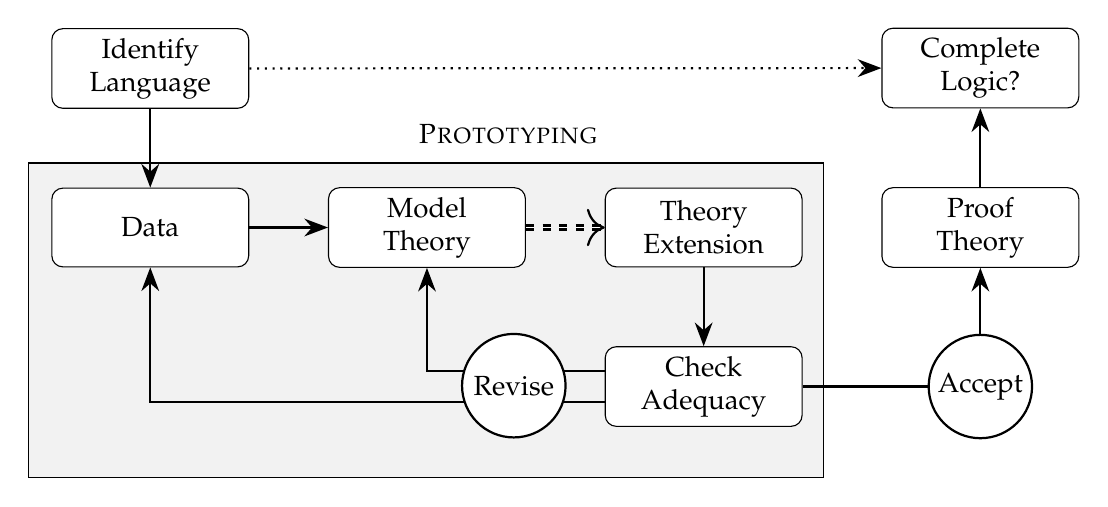
\begin{tikzpicture}[
		node distance=1cm,
		box/.style={
      draw,
      rounded corners,
      minimum width=2.5cm,
      minimum height=1cm,
      align=center,
      fill=white
    },
		arrow/.style={-{Stealth[length=3mm]}, thick}
		]

		\node[box] (lang) {Identify\\Language};

		\coordinate (core_pos) at ([xshift=-1.25cm,yshift=-1.5cm]lang);
		\coordinate (check_pos) at ([xshift=9.5cm,yshift=-3.4cm]core_pos);
		\node[above] at ([yshift=0.3cm]core_pos -| {$(core_pos)!0.5!(check_pos)$}) {\sc \strut\hspace{2cm} Prototyping};
		\draw[fill=gray!10] ([shift={(-0.3,0.3)}]core_pos) rectangle ([shift={(0.3,-0.3)}]check_pos);

		\node[box, below=of lang] (data) {Data};
		\node[box, right=of data] (model) {Model\\Theory};
		\node[box, right=of model] (ext) {Theory\\Extension};
		\node[box, below=of ext] (check) {Check\\Adequacy};
		\node[box, right=of ext] (proof) {Proof\\Theory};
		\node[box, above=of proof] (complete) {Complete\\Logic?};

		\draw[arrow] (lang) -- (data);
		\draw[arrow] (data) -- (model);
		\draw[arrow, double, dashed, ->] (model) -- (ext);
		\draw[arrow] (check) -| node[circle,draw,fill=white,pos=0.5,inner sep=2pt] {Accept} (proof);
		\draw[arrow] (proof) -- (complete);
		\draw[arrow] (ext) -- (check);
		\coordinate (check_up) at ([yshift=.2cm]check.west);
		\coordinate (check_down) at ([yshift=-.2cm]check.west);
		\draw[arrow] (check_up) -| (model);
		\draw[arrow] (check_down) -| node[circle,draw,fill=white,pos=0.1,inner sep=3pt,yshift=6pt] {Revise} (data);
		\draw[arrow, dotted] (lang) -- (complete);

	\end{tikzpicture}
\end{center}



\section*{Difficulties}%

\nicebox{
	The standard methodology has the following drawbacks:
	\begin{itemize}
		\item Computationally grueling to prototype semantic theories
		\item Problems of accuracy, redundancy, and memory
		\item Limits complexity in the development of semantic theories
		\item Restricts which language fragments can be studied/combined
	\end{itemize}
}


\section*{An Extended Methodology}%

\nicebox{
	Humans should not be carrying the computational load.
	\begin{itemize}
		\item SAT solvers, SMT solvers, Z3
		\item Inequalities, bitvectors as states
		\item Truth-conditions as Z3 constraints
	\end{itemize}
}

\vspace{-.2in}

\begin{center}
	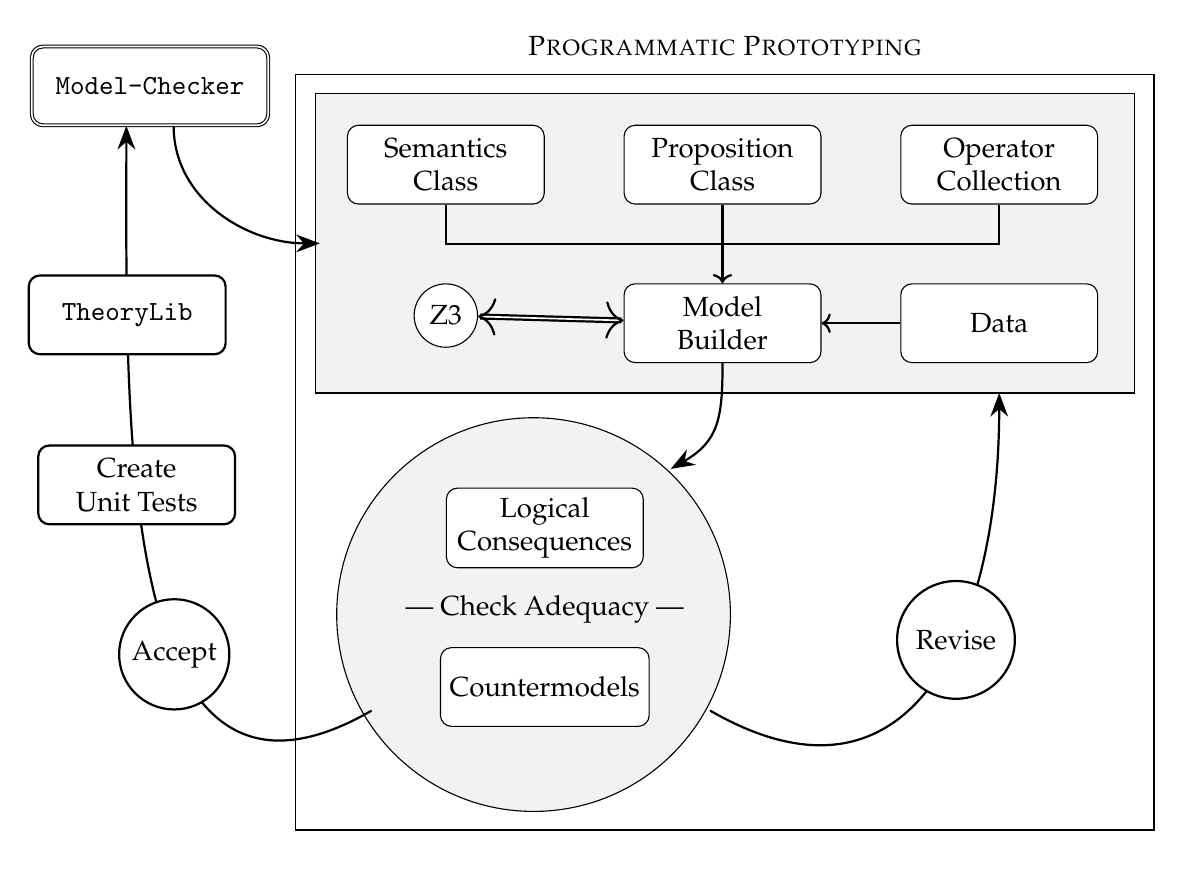
\begin{tikzpicture}[
		node distance=1cm,
		box/.style={
      draw,
      rounded corners,
      minimum width=2.5cm,
      minimum height=1cm,
      align=center,
      fill=white
    },
		arrow/.style={-{Stealth[length=3mm]}, thick}
		]

		\node[box, double] (model) {\tt ~Model-Checker~};

		\coordinate (below_model) at ([xshift=1.5cm,yshift=-1cm]model);
		\coordinate (core_pos) at ([xshift=2.4cm,yshift=-.4cm]model);
		\coordinate (check_pos) at ([xshift=9.8cm,yshift=-3.2cm]core_pos);
		\coordinate (big_top) at ([xshift=-.25cm,yshift=.25cm]core_pos);
		\coordinate (big_bot) at ([xshift=10.3cm,yshift=-9cm]big_top);
		\node[above] at ([yshift=0.4cm]big_top -| {$(core_pos)!0.5!(check_pos)$}) {\sc Programmatic Prototyping};
		\draw ([shift={(-0.3,0.3)}]big_top) rectangle ([shift={(0.3,-0.3)}]big_bot);
		\draw[fill=gray!10] ([shift={(-0.3,0.3)}]core_pos) rectangle ([shift={(0.3,-0.3)}]check_pos);

		\node[box, right=of below_model] (sem) {Semantics\\Class};
		\node[circle, draw, align=center, fill=white, below=of sem] (z3) {Z3};
		\node[box, right=of sem] (prop) {Proposition\\Class};
		\node[box, right=of prop] (ops) {Operator\\Collection};
		\node[box, below=of prop] (build) {Model\\Builder};
		\node[box, right=of build] (exp) {Data};

		\coordinate (below) at ([yshift=-2.6cm]build);
		\coordinate (top_left) at ([xshift=-4cm,yshift=.9cm]below);
		\coordinate (bot_right) at ([xshift=3.2cm,yshift=-4.0cm]top_left);
		\draw[fill=gray!10] ($(top_left)!0.5!(bot_right)$) ellipse (2.5cm and 2.5cm);
		% \node[below] at ($(top_left)!0.5!(bot_right) + (0,-2.8cm)$) {Check Adequacy};


		\node[box, left=of below] (thrm) {Logical\\Consequences};
		\node[below=0.22cm of thrm] (adeq) {--- Check Adequacy ---};
		\node[box, below=of thrm] (count) {Countermodels};
		\coordinate (revise) at ([yshift=-4.5cm]ops);
		% \node[box, below=of revise] (check) {Revise\\Semantics};

		\coordinate (box_in) at ([xshift=-1.6cm,yshift=-1cm]sem);
		\coordinate (model_out) at ([xshift=.3cm]model.south);
		\draw[arrow] (model_out) to[out=270,in=180] (box_in);

		\coordinate (cir_in) at ([xshift=1.6cm,yshift=.75cm]thrm);
		\draw[arrow] (build.south) to[out=-90,in=30,looseness=1.2] (cir_in);

		\draw[arrow, ->] (exp) -- (build);
		\coordinate (cir_out) at ([xshift=-2.2cm,yshift=-.3cm]count);
		\coordinate (model_in) at ([xshift=-.3cm]model.south);
		\draw[arrow] (cir_out) to[out=210,in=-90,looseness=1.2]
		node[box,draw,fill=white,pos=0.8,inner sep=3pt] {\tt TheoryLib}
		node[box,draw,fill=white,pos=0.62,inner sep=3pt] {Create\\Unit Tests}
		node[circle,draw,fill=white,pos=0.4,inner sep=3pt] {Accept}
		(model_in);

		\coordinate (cir_right) at ([xshift=4.3cm]cir_out);
		\coordinate (box_right) at ([yshift=-2.9cm]ops);
		\draw[arrow] (cir_right) to[out=-30,in=-90,looseness=1.4] node[circle,draw,fill=white,pos=0.6,inner sep=5pt] {Revise} (box_right);

		\draw[arrow, ->] (prop) -- (build);
		\draw[thick] (sem.south) |- ([yshift=.5cm]build.north);
		\draw[thick] (ops.south) |- ([yshift=.5cm]build.north);
		\draw[arrow, double, <->] (z3) -- (build);

	\end{tikzpicture}
\end{center}

\vspace{-20pt}

\section*{Conceptual Engineering}%

\nicebox{
	This methodology has the following advantages:
	\begin{itemize}
		\item Efficiently prototype new semantic theories
		\item Modular semantics, theory of propositions, operators
		\item Evaluate unified languages with many operators
		\item Compare rival theories over large data sets
	\end{itemize}
	Give it a try at: \href{https://pypi.org/project/model-checker/}{\texttt{https://pypi.org/project/model-checker/}}
}


\vfill

\bibliographystyle{Phil_Review} %%bib style found in bst folder, in bibtex folder, in texmf folder.
\nobibliography{Zotero} %%bib database found in bib folder, in bibtex folder


\end{document}
